In the classification task we have to develop a network which classifies the MNIST dataset, i.e. the dataset containing handwritten
digits from $0$ to $9$. This dataset is quite exhaustive, and so we will not need to apply the Cross-validation technique.
The size of this dataset present nevertheless another challenge: the training time can become too long. For this reason we really
need to finely optimize the number of epochs we use in this procedure. One possible solution would be, as in the previous case,
use them as a hyper parameter. However, we will waste a lot of computational resources in this search. We so decided to apply
a technique that is called early stopping: if the validation loss $l_{v}$ does not diminish sufficiently in a given number of
epochs then we kill the training loop. In this way we can get rid of poorly initialized networks and have an overall speed up
of the process. In particular, calling $\vec{l}^{(t)}=(l_{v}^{(1)},l_{v}^{(2)}, \dots, l_{v}^{(t)} )$ the vector containing all the losses at iteration $t$, with a maximum number
of iteration $T$ we stop the process if:
\begin{equation}
    \bar{l} - l_v^{(t)} < 0.01 \hspace{0.5 cm} \mbox{with } \begin{cases}\bar{l}= \frac{1}{t-\tau}\sum_{i=\tau}^t l_v^{(i)} \\ \tau=\min(t, T/10)
    \end{cases}
\end{equation}

The other main difference with respect to the regression task is that the dataset is composed by images. For this reason we 
decided to use two convolutional layers at the beginning of the network. These layers make use of filters, i.e. feature maps
that are applied along all the image with the same weights. We will use filters of dimension $3\times3$. This means that we
will several small $3\times3$ feature maps that will enhance the same details along all the figure. The remarkable example 
in this framework are filters which enhance edges. We will analyze them in Section \ref{sec:res_class}.

Through a random search we will optimize the following parameters:
\begin{itemize}
    \item The dropout;
    \item The learning rate;
    \item The optimizer, choosing from stochastic gradient descent and Adam;
    \item the strength of the L2 regularization,
\end{itemize}

To further enhance the dataset we will apply a random rotation of $45°$ and some Gaussian noise. To help the network in the learning
phase we will also normalize the inputs, using the apposite pytorch transformation. We present the network structure in Figure \ref{fig:cl_net}
\begin{figure}[h]
    \centering
    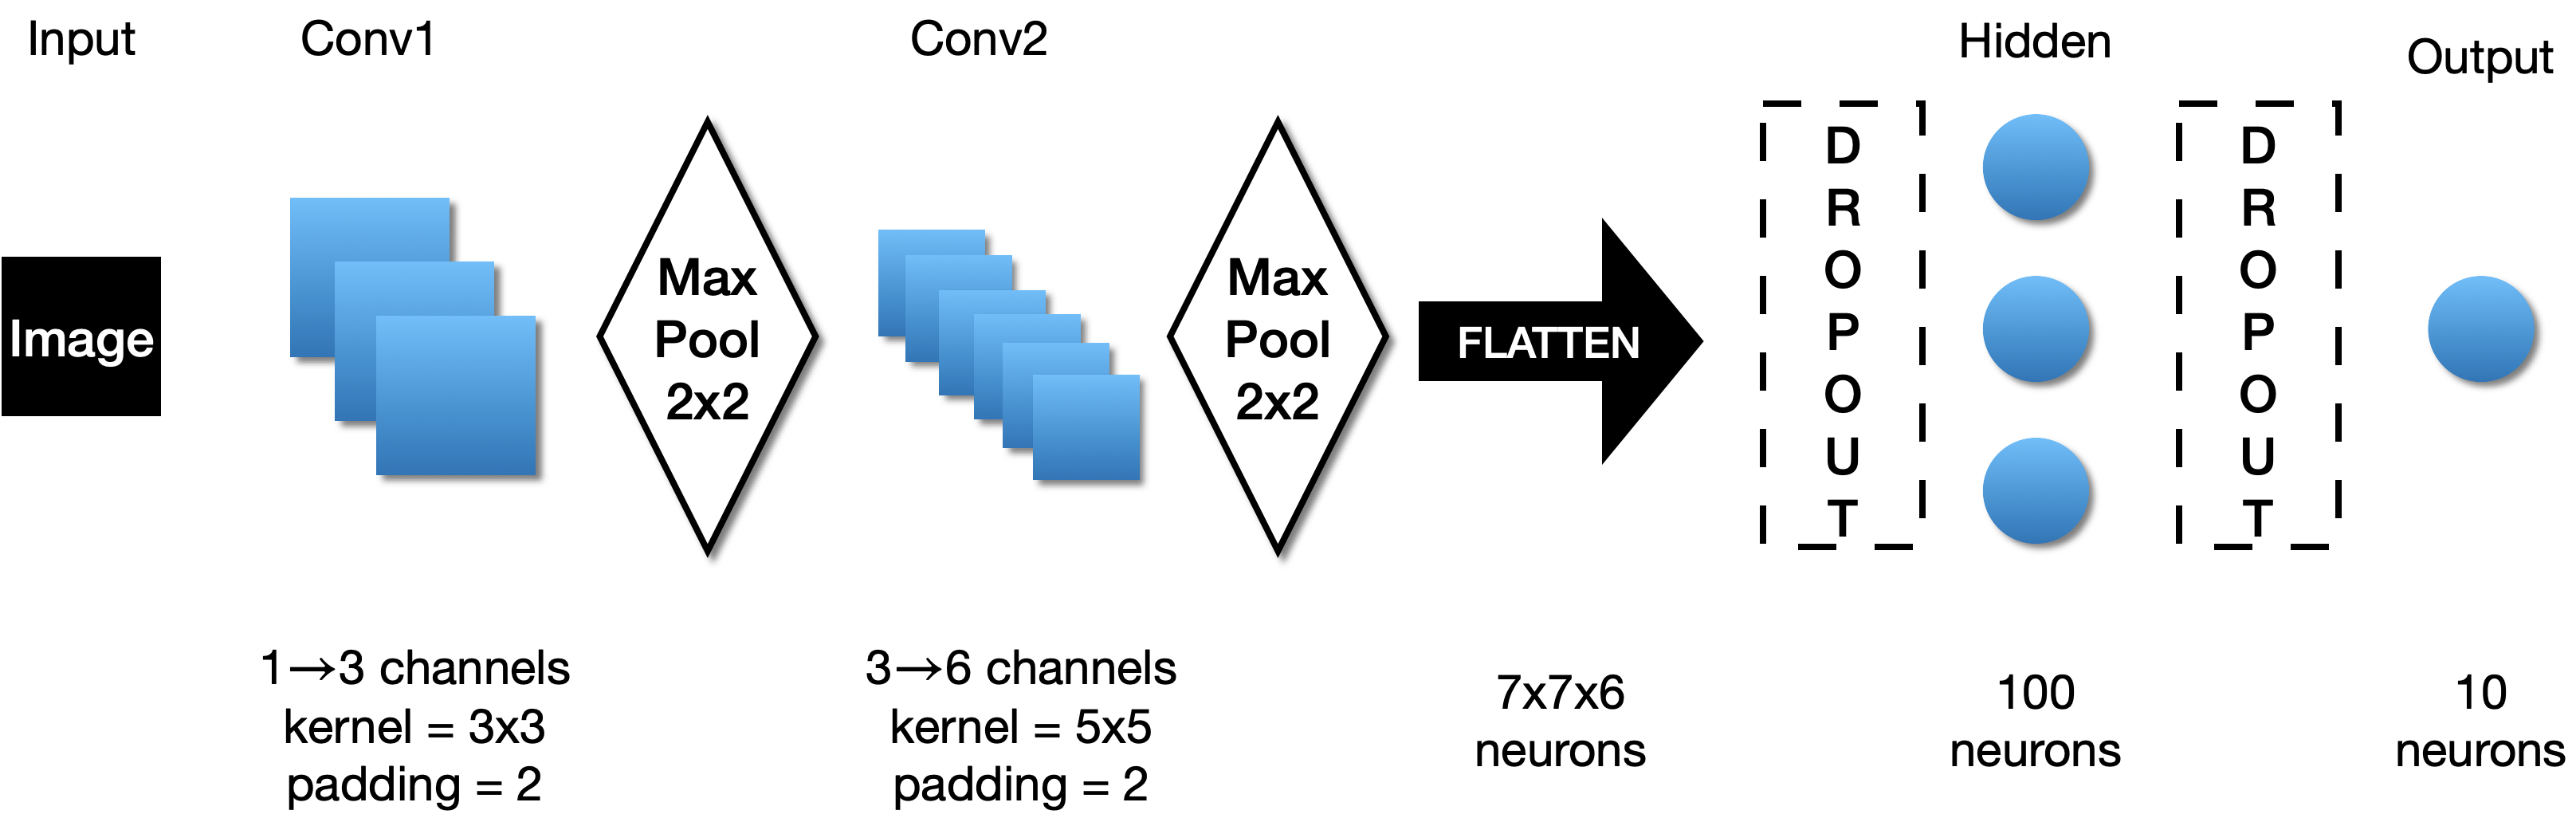
\includegraphics[width=0.8\textwidth]{Images/clas_net.png}
    \caption{Network structure for the classification task. The activation function used is the rectified linear unit.
    The output digit is selected as the argmax among the $10$ output neurons.}
    \label{fig:cl_net}
\end{figure}